\documentclass[11pt,a4paper]{article}
\usepackage[margin=2.4cm]{geometry}
\usepackage[T1]{fontenc}
\usepackage[utf8]{inputenc}
\usepackage{lmodern}
\usepackage{amsmath,amssymb,bm}
\usepackage{siunitx}
\sisetup{per-mode=symbol,separate-uncertainty=true}
\usepackage{booktabs}
\usepackage{graphicx}
\usepackage{caption}
\usepackage{subcaption}
\usepackage{tikz}
\usetikzlibrary{positioning,arrows.meta,shapes.geometric,fit}
\usepackage{xcolor}
\usepackage{hyperref}
\usepackage{enumitem}
\usepackage{listings}
\usepackage{microtype}
\hypersetup{colorlinks=true,linkcolor=blue!50!black,citecolor=blue!50!black,urlcolor=blue!50!black}
\graphicspath{{../figures/}}

\definecolor{sfblue}{HTML}{2A78D6}
\definecolor{sforange}{HTML}{EB6834}
\definecolor{sfgray}{HTML}{898781}
\lstset{basicstyle=\ttfamily\small,columns=fullflexible,keepspaces=true,breaklines=true,
  frame=single,framerule=0.3pt,rulecolor=\color{sfgray},xleftmargin=4pt,xrightmargin=4pt}

\newcommand{\dv}{\Delta v}
\newcommand{\vinf}{v_\infty}
\newcommand{\code}[1]{\texttt{#1}}
\newcommand{\pkg}{\code{mission\_analysis}}

\title{\textbf{A Patched-Conic Mission Analysis Tool for Lunar and Interplanetary Design}\\[4pt]
\large Modeling approach, validation, utility and limitations\\[2pt]
\normalsize \code{sfmission} (\code{sfmission}) v0.1}
\author{MECE 4305 Mechanics \& Thermodynamics of Propulsion --- Rocket Module, Week 10\\
Columbia University, Fall 2026}
\date{9 November 2026}

\begin{document}
\maketitle

\begin{abstract}
\noindent
This report documents \pkg{}, a Python package (with a command-line interface and a Model
Context Protocol server) for preliminary design of lunar and interplanetary missions. The
tool implements the first four steps of the rocket-module design roadmap---mission definition,
required $\dv$, propellant mass fraction and required $I_{sp}$, staging---using patched-conic
astrodynamics with analytic ephemerides: Hohmann and Lambert transfers, porkchop launch-window
maps, planetocentric departure and capture burns, unpowered and powered gravity assists, the
Bate--Mueller--White Earth--Moon patched conic, launch $\dv$ with site-rotation credit and loss
bands, aerocapture and aerobraking credits, the rocket equation and closed-form optimal
multistage sizing, and $\dv$ budgets that resolve directly into propellant masses. An 85-case
test suite verifies the implementation against textbook examples, an independent ephemeris,
and flown missions: Mars~2020 (heliocentric path length \SI{470.9}{Mkm} vs.\ \SI{\approx 471}{Mkm}
published), Voyager~2's Jupiter flyby, and Apollo~11's translunar coast (68--73~h vs.\ 73.0~h).
We state the modeling assumptions explicitly, quantify their consequences where we can, and
identify a factor-$\sqrt{2}$ discrepancy between the straight-line aerobraking formula used in
the lecture notes and a gravity-aware form confirmed by direct integration. The limitations
section describes what the tool does \emph{not} model and when a higher-fidelity method is required.
\end{abstract}

\setcounter{tocdepth}{1}
\tableofcontents
\clearpage

%==================================================================
\section{Purpose and scope}
%==================================================================
The rocket module organizes its lectures and the team project around a ten-step design
procedure (Sutton~\cite{sutton}): mission definition $\rightarrow$ required $\dv$ $\rightarrow$
propellant mass fraction $\rightarrow$ required $I_{sp}$ $\rightarrow$ staging/architecture
$\rightarrow$ stage thrust $\rightarrow$ single-point thrust-chamber design $\rightarrow$
$\dot m$, $V_e$ $\rightarrow$ $p_c$, $M_e$, $A_e$, $T_c$ $\rightarrow$ feed system
$\rightarrow$ iterate. The tool described here covers steps~1--4 and is intended to be:

\begin{enumerate}[nosep]
\item a \textbf{lecture instrument} for Week~10 (\emph{Mission Analysis}): live porkchop
      plots of the Earth--Mars window opening this month, Earth--Moon transfers, and the
      $\dv$ levers (aerobraking, retro-propulsion, gravity assists);
\item the \textbf{reference solution for HW~1} (mission $\dv$ budget and staging) and the
      first module of each team's project model;
\item a \textbf{preliminary-design tool} in its own right, exposed to agents through MCP so
      that it can be composed with the course's thermochemistry, nozzle and cycle models.
\end{enumerate}

\paragraph{Fidelity class.} The tool is a \emph{patched-conic, impulsive-burn} model with
\emph{analytic mean-element ephemerides}. It is the appropriate fidelity for sizing a
propulsion system and for understanding why a mission's $\dv$ is what it is. It is not a
trajectory-design tool: it does not propagate perturbed motion, does not model finite burns,
and does not target B-plane conditions. Section~\ref{sec:limits} makes these boundaries precise.

\paragraph{Interfaces.} The same functions are available as a Python API, a CLI and 23 MCP
tools returning JSON, so that a design agent can request, e.g., a Mars-orbiter $\dv$ budget on
specific dates and hand the injected mass to a staging or engine-sizing tool:
\begin{lstlisting}
from sfmission import porkchop, interplanetary_budget
sfmission porkchop Earth Mars 2026-09-01 2027-02-15 --tof 120 450 --plot pork.png
sfmission-mcp        # MCP server (stdio); tools listed in Appendix B
\end{lstlisting}

%==================================================================
\section{Architecture}
%==================================================================
Figure~\ref{fig:arch} shows the module dependency graph. Low-level modules work in
\si{km}, \si{s}, \si{rad}; high-level functions accept altitudes in \si{km}, angles in degrees
where the argument name ends in \code{\_deg}, and epochs as \code{datetime}, ISO-8601 strings
or Julian Dates.

\begin{figure}[h]
\centering
\resizebox{\textwidth}{!}{%
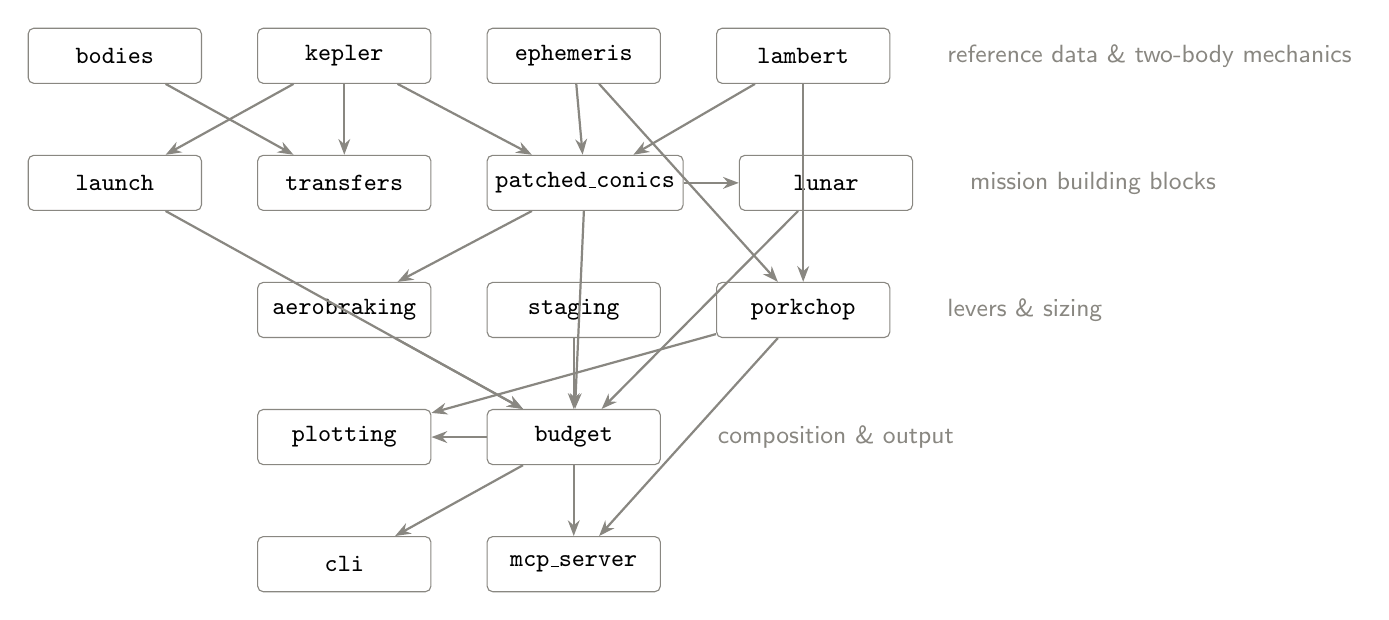
\begin{tikzpicture}[
  box/.style={draw=sfgray,rounded corners=2pt,fill=white,minimum height=7mm,minimum width=22mm,font=\small\ttfamily,inner sep=3pt},
  lay/.style={font=\small\sffamily\color{sfgray},anchor=west},
  arr/.style={-{Stealth[length=2mm]},draw=sfgray,thick},
  node distance=5mm and 7mm]
\node[box] (bodies) {bodies};
\node[box,right=of bodies] (kepler) {kepler};
\node[box,right=of kepler] (eph) {ephemeris};
\node[box,right=of eph] (lam) {lambert};
\node[box,below=9mm of kepler] (tr) {transfers};
\node[box,right=of tr] (pc) {patched\_conics};
\node[box,right=of pc] (lun) {lunar};
\node[box,left=of tr] (launch) {launch};
\node[box,below=9mm of tr] (aero) {aerobraking};
\node[box,right=of aero] (stg) {staging};
\node[box,right=of stg] (pork) {porkchop};
\node[box,below=9mm of stg] (bud) {budget};
\node[box,left=of bud] (plot) {plotting};
\node[box,below=9mm of bud] (mcp) {mcp\_server};
\node[box,left=of mcp] (cli) {cli};
\draw[arr] (bodies) -- (tr); \draw[arr] (kepler) -- (tr); \draw[arr] (kepler) -- (pc); \draw[arr] (eph) -- (pc);
\draw[arr] (lam) -- (pc); \draw[arr] (kepler) -- (launch); \draw[arr] (pc) -- (lun); \draw[arr] (pc) -- (aero);
\draw[arr] (eph) -- (pork); \draw[arr] (lam) -- (pork); \draw[arr] (pc) -- (bud); \draw[arr] (lun) -- (bud);
\draw[arr] (launch) -- (bud); \draw[arr] (aero) -- (bud); \draw[arr] (stg) -- (bud); \draw[arr] (pork) -- (plot);
\draw[arr] (bud) -- (plot); \draw[arr] (bud) -- (mcp); \draw[arr] (bud) -- (cli); \draw[arr] (pork) -- (mcp);
\node[lay] at ([xshift=6mm]lam.east) {reference data \& two-body mechanics};
\node[lay] at ([xshift=6mm]lun.east) {mission building blocks};
\node[lay] at ([xshift=6mm]pork.east) {levers \& sizing};
\node[lay] at ([xshift=6mm]bud.east |- bud) {composition \& output};
\end{tikzpicture}}
\caption{Module dependency graph (arrows point from dependency to dependent). Everything above the
\code{budget} layer is pure functions returning dataclasses; the three front ends only format.}
\label{fig:arch}
\end{figure}

%==================================================================
\section{Modeling approach}
%==================================================================

\subsection{Reference data}
Gravitational parameters are the JPL DE440 values~\cite{de440,astropar} (planet-\emph{system}
GMs for the outer planets, which is what a flyby of the system sees); radii are IAU nominal
values. Spheres of influence use the Laplace form $r_{SOI}=a\,(m/M)^{2/5}$.

Planetary positions come from JPL's \emph{Keplerian Elements for Approximate Positions of the
Major Planets}~\cite{standish}: six elements and their secular rates, Table~1 valid
1800--2050 (default) and Table~2a/2b valid 3000~BC--3000~AD (used automatically outside Table~1,
with the extra $M$ terms for Jupiter--Neptune). Elements are referred to the J2000 ecliptic;
velocities are the two-body velocities on the instantaneous mean orbit (the secular element
rates contribute $<\SI{1e-6}{km/s}$). ``Earth'' is the Earth--Moon barycenter unless the
Moon correction is requested. The Moon is a truncated Meeus series~\cite{meeus} (32
longitude/distance and 20 latitude terms plus the planetary additive terms), precessed from
the ecliptic of date to J2000 by the general precession in longitude.

Table~\ref{tab:eph} compares these models with an independent one (astropy's built-in
ERFA \code{plan94}/\code{moon98} ephemeris). The agreement is within the accuracy JPL quotes for
the tables; for mission design the consequence is a $\vinf$ error of order \SI{1}{m/s} at
Earth and \SI{\sim 10}{m/s} at Saturn---negligible against the $\dv$ margins of a budget.

\begin{table}[h]\centering\small
\caption{Analytic ephemeris vs.\ astropy built-in ephemeris, four epochs 2000--2045 (worst case).}
\label{tab:eph}
\begin{tabular}{lccc}\toprule
Body & angle [$''$] & rel.\ distance & velocity [m/s] \\\midrule
Mercury, Venus, Earth(--Moon bary.), Mars & $<35$ & $<\num{1.5e-4}$ & $<5$ \\
Jupiter & $<340$ & $<\num{4e-4}$ & $<28$ \\
Saturn & $<560$ & $<\num{1.5e-3}$ & $<41$ \\
Uranus, Neptune & $<110$ & $<\num{1e-3}$ & $<16$ \\
Moon (geocentric) & $<40$ & $<\SI{40}{km}$ & -- \\\bottomrule
\end{tabular}
\end{table}

\subsection{Two-body mechanics}
\code{kepler} provides the vis-viva relation $v^2=\mu(2/r-1/a)$, classical elements from and
to state vectors (Curtis~\cite{curtis} Algorithms~4.2/4.5), Kepler's equation (Newton from
Danby's starting value with a bisection fallback), and universal-variable propagation
(Curtis Algorithm~3.4) valid for all conics. Hyperbola relations used by the patched-conic
modules are
\begin{equation}
 v_p=\sqrt{\vinf^2+\frac{2\mu}{r_p}},\qquad e=1+\frac{r_p\vinf^2}{\mu},\qquad
 \delta=2\arcsin\frac1e,\qquad \Delta=r_p\sqrt{1+\frac{2\mu}{r_p\vinf^2}},
\end{equation}
for periapsis speed, eccentricity, asymptotic turning angle and aiming radius.

\subsection{Lambert's problem}
The heliocentric leg between two ephemeris positions is the single-revolution Lambert
solution in the universal-variable formulation~\cite{bmw,curtis}: with
$A=\sin\Delta\theta\sqrt{r_1 r_2/(1-\cos\Delta\theta)}$ and $y(z)=r_1+r_2+A\,(zS(z)-1)/\sqrt{C(z)}$,
\begin{equation}
F(z)=\Big[\frac{y(z)}{C(z)}\Big]^{3/2}S(z)+A\sqrt{y(z)}-\sqrt{\mu}\,\Delta t=0 .
\end{equation}
$F$ is monotonic in $z$ on the single-revolution branch, so the root is bracketed
(hyperbolic side $z<0$ to the $z\to 4\pi^2$ limit, after locating $y=0$ when $A<0$) and
solved with Brent's method; this never diverges, unlike a bare Newton iteration, and both
type-I ($\Delta\theta<\pi$) and type-II ($\Delta\theta>\pi$) transfers fall out of the
geometry for prograde motion. A solve costs $\approx\SI{55}{\micro s}$; a $110\times110$
porkchop grid takes about a second. The $\Delta\theta=\pi$ singularity (undefined transfer
plane) is reported as an exception and shows up as the familiar ridge in porkchop plots.

\subsection{Patched conics}
Departure from a circular parking orbit of radius $r_p$ onto a hyperbola with excess speed
$\vinf=|\bm v_{sc}-\bm v_{planet}|$ costs $\dv=\sqrt{\vinf^2+2\mu/r_p}-\sqrt{\mu/r_p}$;
capture into an orbit with apsides $(r_p,r_a)$ costs $\dv=\sqrt{\vinf^2+2\mu/r_p}-
\sqrt{\mu(2/r_p-2/(r_p+r_a))}$. Both are tangential periapsis burns, the optimum for
impulsive maneuvers.

An \textbf{unpowered flyby} rotates $\bm\vinf$ by $\delta$ about the normal to the
$(\bm v_{planet},\bm\vinf)$ plane; the heliocentric speed change is $|\dv|=2\vinf\sin(\delta/2)$.
For multi-leg sequences (Earth--Venus--Mars, Earth--Mars--Earth--Jupiter, \dots) the incoming
and outgoing $\bm\vinf$ from the adjacent Lambert legs generally differ in both direction and
magnitude. The tool uses the standard \textbf{powered-flyby} model of the multiple-gravity-assist
(MGA) literature~\cite{izzo}: a common periapsis radius $r_p$ is found such that
$\tfrac12\delta(\vinf^{in},r_p)+\tfrac12\delta(\vinf^{out},r_p)=\angle(\bm\vinf^{in},\bm\vinf^{out})$,
and the speed mismatch is made up by a tangential burn at periapsis,
$\dv=\big|\sqrt{(\vinf^{out})^2+2\mu/r_p}-\sqrt{(\vinf^{in})^2+2\mu/r_p}\big|$. If the required
turning cannot be achieved above a minimum altitude the flyby is flagged infeasible. This
charges the right order of magnitude for ``almost-free'' assists (Voyager~2 at Jupiter:
\SI{0.05}{km/s}, Section~\ref{sec:val}) while making infeasible sequences visible.

\subsection{Porkchop maps}
A grid of departure dates $\times$ times of flight is solved leg by leg; each cell records
$C_3=\vinf^2$ at departure, $\vinf$ at arrival, the transfer angle, and the departure and
capture $\dv$ for the requested parking and capture orbits. The grid optimum, the launch
window at a chosen $\dv$ threshold, and the equatorial declination of the launch asymptote
(DLA) are derived quantities. Figure~\ref{fig:pork} is the Earth--Mars window opening in
October~2026.

\begin{figure}[t]\centering
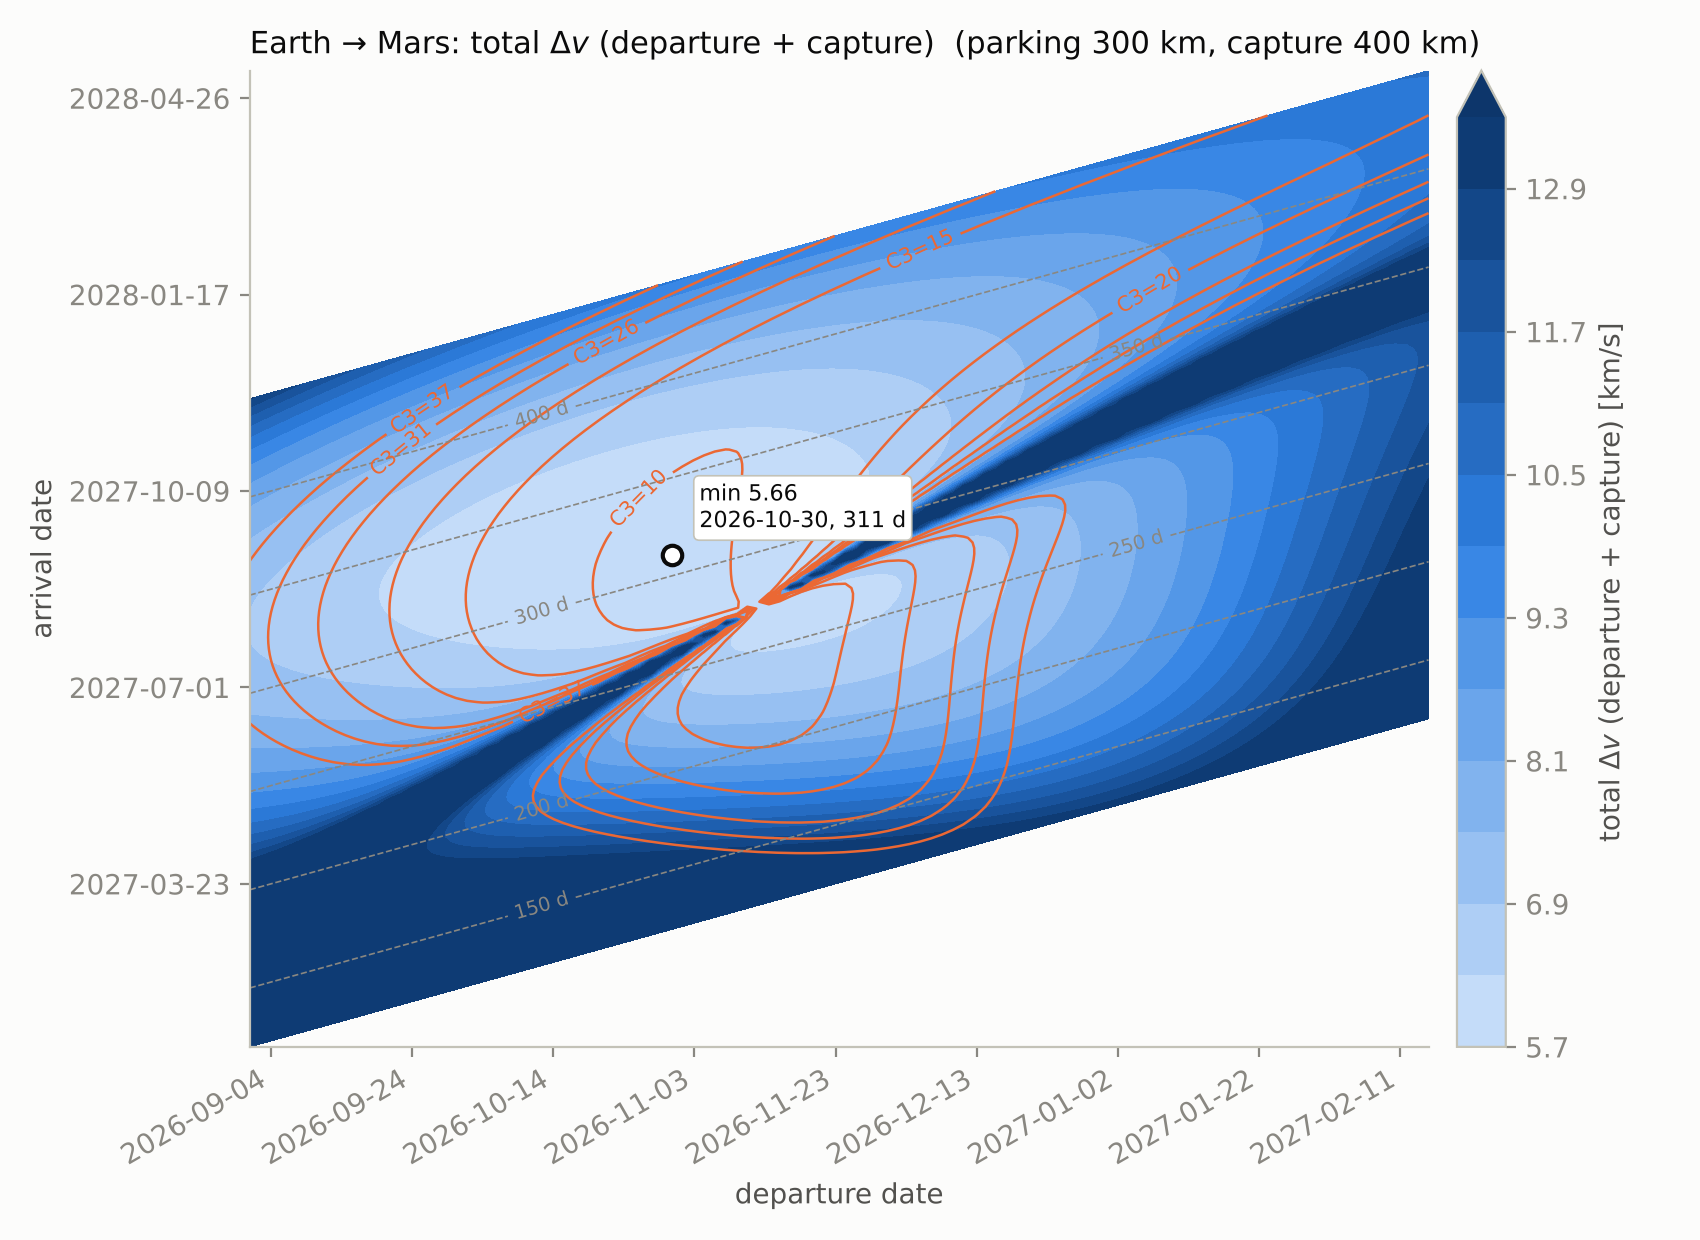
\includegraphics[width=0.78\textwidth]{porkchop_earth_mars_2026_dvtotal}
\caption{Earth$\to$Mars 2026/27: total $\dv$ (departure from a \SI{300}{km} parking orbit plus
capture into a \SI{400}{km} Mars orbit); $C_3$ contours in orange, time of flight dashed.
Optimum: depart 2026-10-30, 311~d type~II, $C_3=\SI{9.2}{km^2/s^2}$, $\vinf^{arr}=\SI{2.57}{km/s}$,
$\dv=\SI{5.66}{km/s}$; the type-I alternative (2026-11-16, 260~d) costs \SI{6.02}{km/s}.}
\label{fig:pork}
\end{figure}

\subsection{Earth--Moon patched conic}
Two levels are provided. The \emph{Hohmann-to-the-Moon} estimate treats the Moon as a point at
the apogee of a transfer ellipse and uses $\vinf=|v_{Moon}-v_{apogee}|$ for lunar orbit
insertion (LOI); it gives the textbook \SI{3.13}{km/s} TLI and \SI{0.82}{km/s} LOI. The
\emph{Bate--Mueller--White} method~\cite{bmw} (\S7.4) patches a geocentric ellipse from the
injection state $(r_0,v_0,\phi_0)$ to the lunar sphere of influence at the point set by the
arrival angle $\lambda_1$, then a selenocentric hyperbola from $\bm v_2=\bm v_1-\bm v_{Moon}$.
We implement the geometry with vectors (Moon at $(D,0)$ moving in $+y$; arrival point
$P=\bm r_{Moon}+r_{SOI}(-\cos\lambda_1,\sin\lambda_1)$), so that the sense of motion about the
Moon follows from the sign of $h_2=(\bm\rho\times\bm v_2)_z$ without the sign ambiguities
of the scalar relations---which are nevertheless reproduced in the tests. Two additions
matter for comparison with flown data: the time spent inside the sphere of influence
(hyperbolic Kepler equation from $r_{SOI}$ to perilune, \SIrange{14}{18}{h} for Apollo-class
approaches) is added to the geocentric time of flight, and a design solver returns the
$\lambda_1$ (for given $v_0$) or $v_0$ (for given $\lambda_1$) that produces a requested
perilune altitude, usually one prograde and one retrograde solution.

\subsection{Launch $\dv$}
\begin{equation}
\dv_{launch}=\big|\bm v_{orbit}-\bm v_{site}\big|+\dv_{grav}+\dv_{drag}+\dv_{steer},\qquad
\bm v_{site}=\omega_\oplus R\cos\varphi\,\hat{\bm e}_E,
\end{equation}
with the launch azimuth from $\cos i=\cos\varphi\sin Az$.
The vector difference accounts for the launch azimuth needed for the target inclination;
due east ($i=\varphi$) it reduces to $v_{circ}-\omega R\cos\varphi$. Losses are carried as a
band (default gravity 1.0--1.5, drag 0.05--0.15, steering 0.1--0.4~km/s~\cite{sutton}), so a
budget shows $\SI{7.726}{}-\SI{0.409}{}+(1.15\ldots2.05)=\SIrange{8.47}{9.37}{km/s}$ for KSC to
\SI{300}{km}. (This also fixes the sign of the Week-9 slide-32 estimate.)

\subsection{Aerocapture and aerobraking}
Aerocapture replaces the propulsive capture burn by one atmospheric pass; the budget credit is
the full capture $\dv$, less the small apoapsis burn that lifts periapsis out of the atmosphere.
Entry speed at the interface altitude is reported for heating/g-load assessment, which the
tool does not perform.

For aerobraking from a high capture ellipse the tool integrates the apoapsis decay pass by
pass. The per-pass speed loss is derived by treating $\rho=\rho_p\exp[-(r-r_p)/H]$ and
expanding $r-r_p\approx\tfrac12\ddot r_p t^2$ about periapsis:
\begin{equation}
\dv_{pass}=\frac{\rho_pV_p^2}{2\beta}\sqrt{\frac{2\pi H}{\ddot r_p}},\qquad
\ddot r_p=\frac{V_p^2}{r_p}-\frac{\mu}{r_p^2},\qquad \beta=\frac{m}{C_DA}.
\label{eq:aero}
\end{equation}
Taking $\ddot r_p=V_p^2/r_p$ (a straight-line fly-through, gravity neglected) gives the
compact form $\rho_pV_p\sqrt{2\pi Hr_p}/(2\beta)$ that appears on the Week-11 slide. The two
differ by $\sqrt{V_p^2/(V_p^2-\mu/r_p)}$, which is $\sqrt2$ for a parabolic pass and larger for
lower apoapses. Direct integration of the planar two-body-plus-drag equations
(\path{aerobraking_pass_dv_numeric}) confirms Eq.~\eqref{eq:aero} to within 0.2\% across
apoapsis altitudes from \SI{2000}{} to \SI{160000}{km}, while the straight-line form is
30--58\% low (Figure~\ref{fig:aero}). The slide formula should be updated accordingly.

\begin{figure}[t]\centering
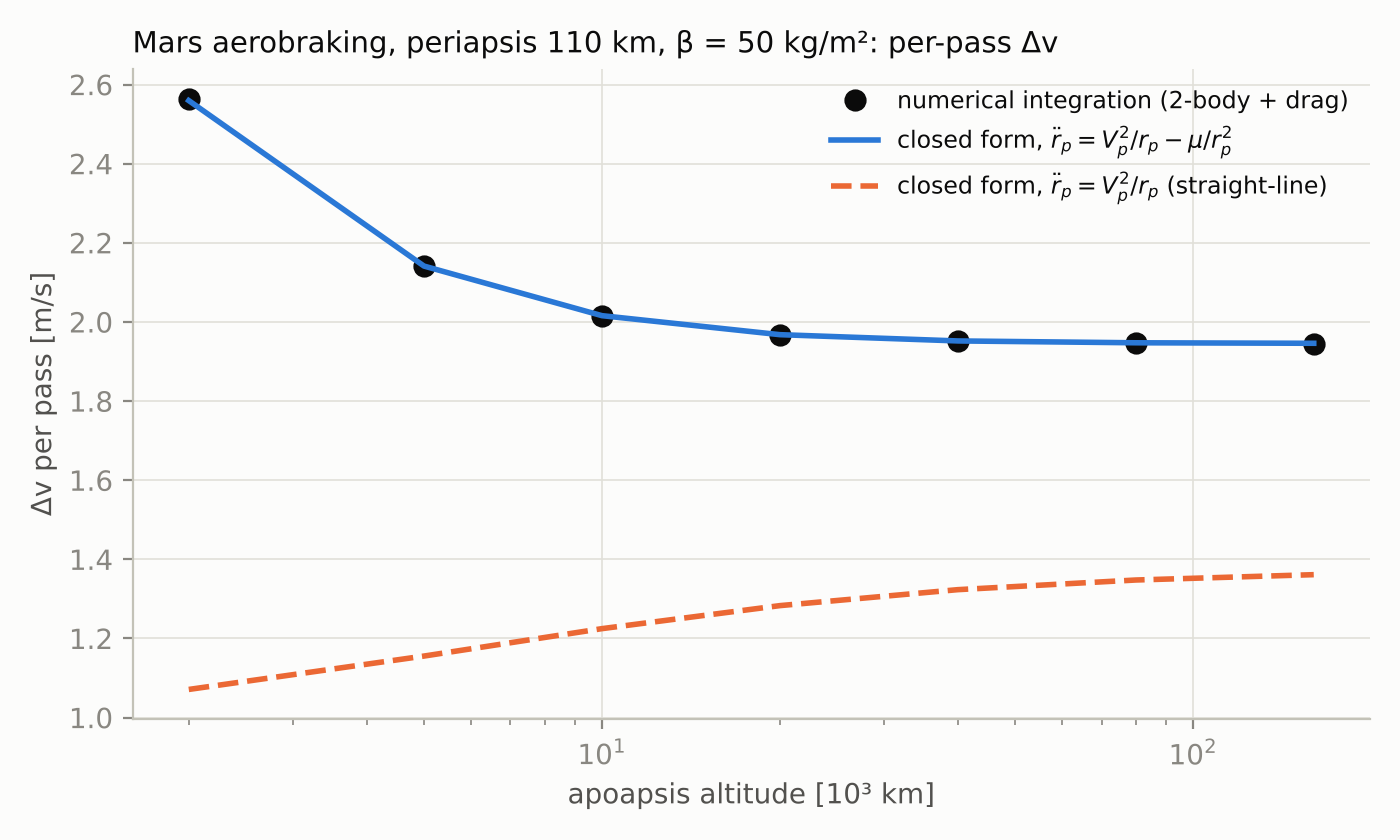
\includegraphics[width=0.7\textwidth]{aerobraking_pass_comparison}
\caption{Per-pass $\dv$ at Mars (periapsis \SI{110}{km}, $\beta=\SI{50}{kg/m^2}$): numerical
integration vs.\ the two closed forms.}
\label{fig:aero}
\end{figure}

\subsection{Rocket equation and staging}
With Sutton's nomenclature,
\[
\zeta=\frac{m_p}{m_0},\qquad MR=\frac{m_f}{m_0},\qquad \sigma_k=\frac{m_{s,k}}{m_{s,k}+m_{p,k}},\qquad
c_k=g_0I_{sp,k},\qquad r_k=e^{\dv_k/c_k}
\]
($\varepsilon$ is deliberately reserved for nozzle area ratio), the initial-to-payload mass
ratio of an $N$-stage vehicle is
\begin{equation}
\frac{m_0}{m_L}=\prod_{k=1}^{N}\frac{r_k(1-\sigma_k)}{1-r_k\sigma_k},
\end{equation}
and the $\dv$ split minimizing $m_0$ for fixed $\sum\dv_k$ follows from a Lagrange multiplier
$\lambda$:
\begin{equation}
r_k=\frac{\lambda c_k-1}{\lambda c_k\sigma_k},\qquad \sum_k c_k\ln r_k=\dv_{tot},
\end{equation}
a single scalar root; identical stages recover the equal-split result. Required $I_{sp}$ for
a given $\zeta$ (roadmap step~3) is $I_{sp}=\dv/[g_0\ln(1/(1-\zeta))]$, and burn sequences are
sized backward from the final mass.

\subsection{Budgets}
A \code{DeltaVBudget} is an ordered list of legs with nominal/low/high values, a kind
(propulsive, aero-assisted, margin) and optionally the $I_{sp}$ of the stage performing the
burn. Composers build budgets for dated interplanetary missions (launch band, injection, powered
flybys, capture or aerocapture, landing, margin) and for lunar missions (launch, TLI, LOI,
Apollo-reference descent/ascent, TEI). Budgets resolve into propellant masses by backward
sizing and report propellant fraction and required $I_{sp}$---the hand-off to the engine
design steps.

%==================================================================
\section{Verification and validation}\label{sec:val}
%==================================================================
The test suite (85 cases, \SI{\sim1}{s}) has three layers: unit checks of the mechanics,
textbook examples with published numbers, and reconstructions of flown missions from their
published dates and states. Table~\ref{tab:val} summarizes them.

\begin{table}[h]\centering\small
\caption{Validation record.}
\label{tab:val}
\begin{tabular}{p{0.46\textwidth}p{0.48\textwidth}}\toprule
Case & Result \\\midrule
Lambert, Curtis Example~5.2 & $\bm v_1,\bm v_2$ to \SI{1e-4}{km/s}; propagation closes to \SI{1e-8}{km}; closure for 20 geometries incl.\ type~II, retrograde and hyperbolic \\
Elements, Curtis Example~4.3 & $h,e,i,\Omega,\omega,\nu$ match \\
Ephemeris vs.\ astropy; Mars oppositions 2022/2025/2027 & Table~\ref{tab:eph}; Earth/Mars longitudes agree $<1.5^\circ$ at opposition \\
Earth$\to$Mars Hohmann (Curtis Ex.~8.4--8.6) & $\vinf$ 2.943/2.648~km/s, $\dv$ 3.590~km/s from \SI{300}{km}, phase angle $44.3^\circ$, synodic period 779.9~d \\
LEO$\to$GEO Hohmann; with $28.5^\circ$ plane change & 3.893~km/s; 4.23~km/s with 26.3$^\circ$ at the apogee burn \\
\textbf{Mars 2020} (launch 2020-07-30 11:50, entry 2021-02-18 20:37 UTC) & heliocentric path \SI{470.9}{Mkm} vs.\ JPL press kit $\approx$\SI{471}{Mkm}~\cite{m2020}; $C_3=\SI{14.5}{km^2/s^2}$; $\vinf^{arr}=\SI{2.55}{km/s}$ consistent with the quoted entry speed \\
Mars 2020 porkchop & optimum in July 2020 with $C_3<15$ \\
\textbf{Voyager 2} E--J--S dates (1977-08-20, 1979-07-09, 1981-08-25) & Jupiter turn $97^\circ$, closest approach \SI{620000}{km} (actual $\approx$\SI{570000}{km} above the cloud tops), powered correction \SI{0.05}{km/s}; $C_3=105$ (Titan~IIIE-Centaur class) \\
\textbf{Apollo 11} TLI state~\cite{a11} (10.832--10.840~km/s at 323--336~km, FPA $\approx7^\circ$) $\to$ LOI & TLI-to-perilune 68--73~h vs.\ 73.0~h actual; LOI 0.89--0.92~km/s vs.\ 0.891~km/s (into 60$\times$170~nmi) \\
Lunar Hohmann estimate & TLI 3.135~km/s, LOI 0.82~km/s \\
Aerobraking pass, Eq.~\eqref{eq:aero} vs.\ integration & 1.952 vs.\ 1.951~m/s \\
Staging identities, optimal split, SSTO limit & exact \\\bottomrule
\end{tabular}
\end{table}

Two observations from the flown-mission cases are worth recording. First, the Apollo~11 result
is as good as the published altitude datum: the two tabulated TLI states (S-IVB cutoff and
``TLI'' ten seconds later) imply injection energies that differ by \SI{0.04}{km^2/s^2}, and the
lunar time of flight moves by about \SI{5}{h} per \SI{0.1}{km^2/s^2}. This sensitivity is
physical and is a good lecture point. Second, the Mars~2020 path length agreeing to 0.02\% shows
that the heliocentric geometry is right; the remaining uncertainty in such reconstructions is
in the planetocentric phases, which the patched-conic model only approximates.

\begin{figure}[t]\centering
\begin{subfigure}[t]{0.49\textwidth}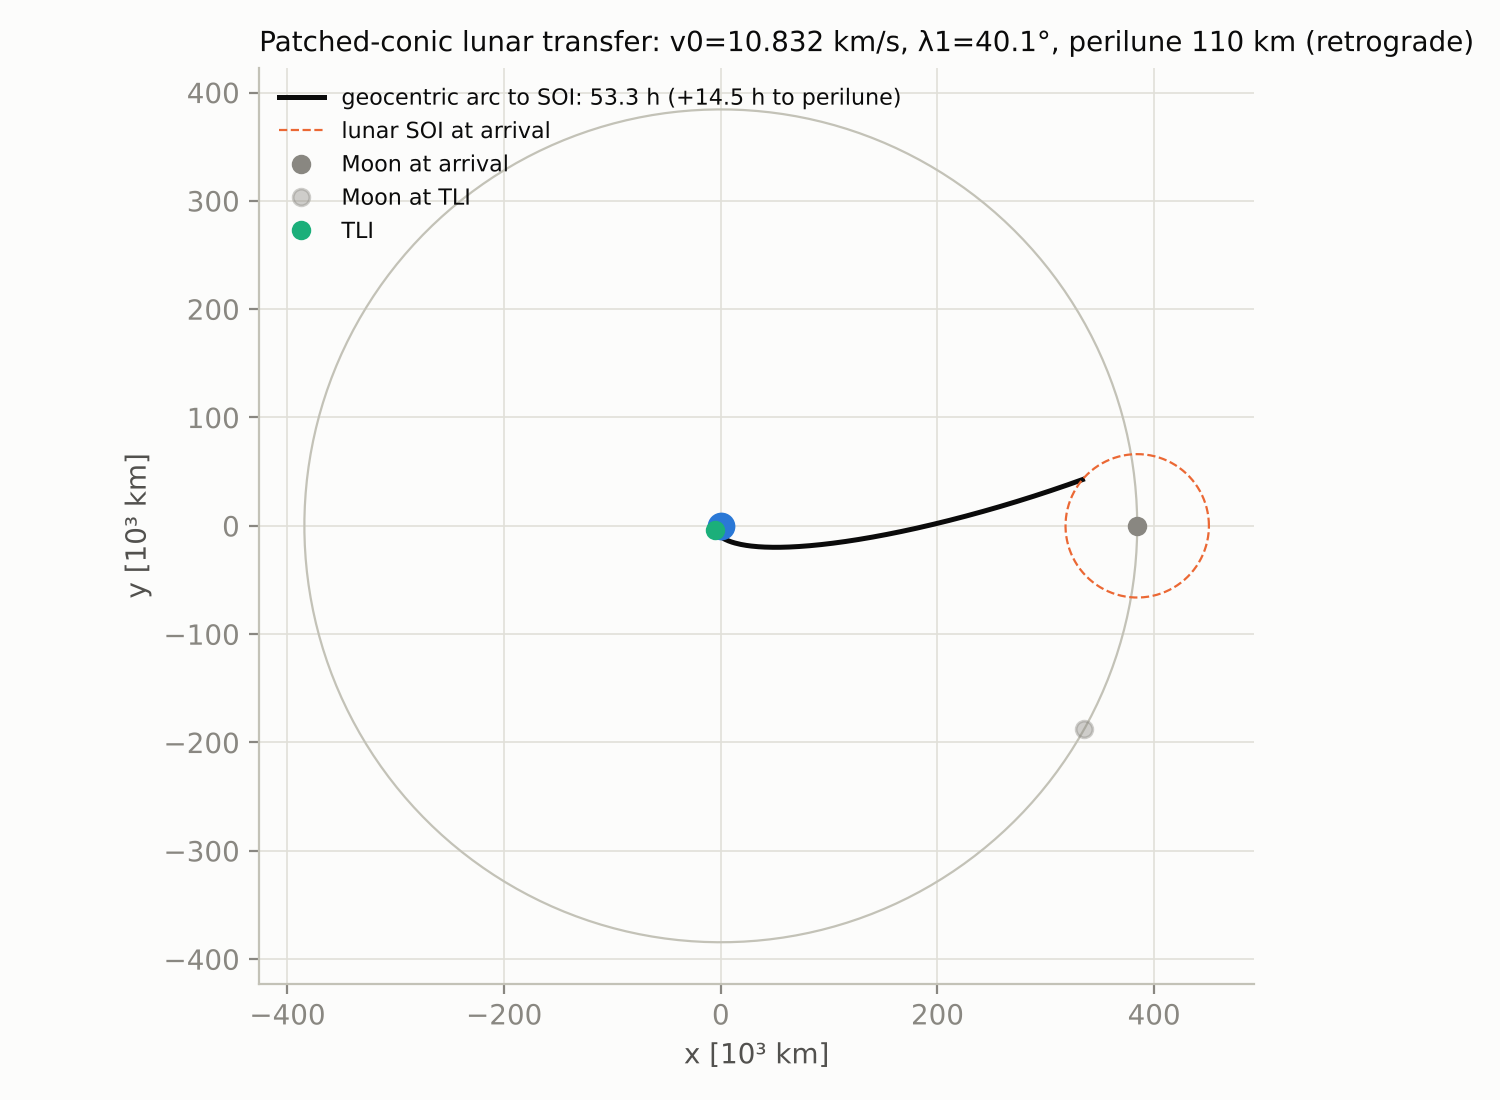
\includegraphics[width=\linewidth]{lunar_patched_conic_apollo11}
\caption{Apollo-11-like patched-conic transfer (plan view, Earth--Moon plane).}\end{subfigure}\hfill
\begin{subfigure}[t]{0.49\textwidth}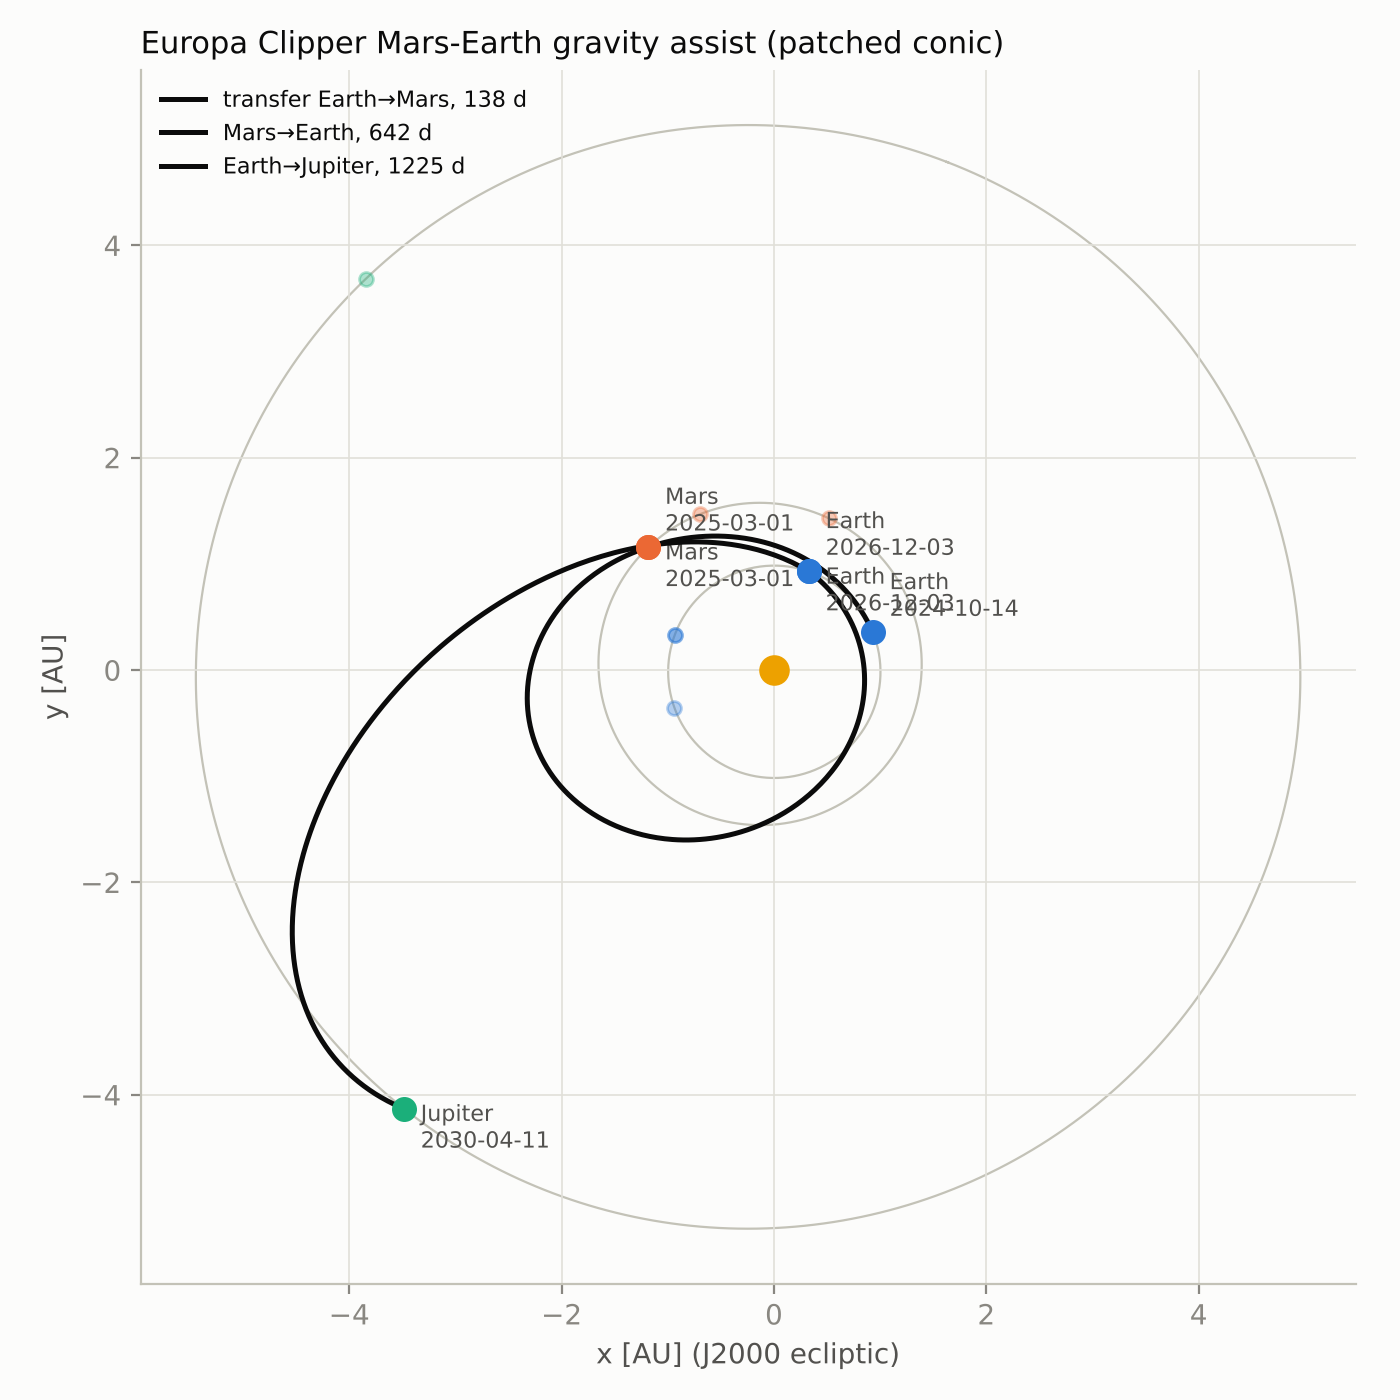
\includegraphics[width=\linewidth]{transfer_europa_clipper_mega}
\caption{Europa Clipper Mars--Earth gravity assist (patched conic on the published dates).}\end{subfigure}
\caption{Geometry outputs used in the Week-10 lecture.}
\end{figure}

%==================================================================
\section{Utility: what the tool is for}
%==================================================================
\paragraph{Lecture.} Figure~\ref{fig:pork} and its companions are generated by
\path{examples/02_mars_porkchop_2026.py} in under a minute, so the Earth--Mars window
opening this month can be shown live, including the current phase angle (56$^\circ$ on
11/12 against the 44.3$^\circ$ Hohmann requirement) and the type-I/type-II trade. The lunar
module shows why a 3-day transfer costs only \SI{20}{m/s} more TLI than the 5-day Hohmann
estimate but \SI{70}{m/s} more LOI, and why retrograde lunar orbits fall out of a leading-side
approach. The aero and gravity-assist modules quantify the levers (Table~\ref{tab:levers}).

\begin{table}[h]\centering\footnotesize
\caption{$\dv$ levers quantified by the tool (Mars arrival $\vinf=\SI{2.65}{km/s}$; Jupiter via Europa Clipper's MEGA dates).}
\label{tab:levers}
\begin{tabular}{p{0.40\textwidth}p{0.24\textwidth}p{0.28\textwidth}}\toprule
Lever & without & with \\\midrule
Aerocapture into \SI{400}{km} Mars orbit & 2.08~km/s & 0.06~km/s (periapsis raise) \\
Aerobraking \SI{110}{}$\times$\SI{40000}{km} $\to$ circular \SI{400}{km}, $\beta=\SI{50}{kg/m^2}$ & 2.08~km/s & 0.92~km/s propulsive; 521 passes, 152~d \\
Mars--Earth gravity assist to Jupiter & $C_3=77$, injection 6.30~km/s, 2.7~yr & $C_3=41$, injection 4.95~km/s, 5.5~yr \\
Launch-site rotation credit, KSC due east vs.\ polar & 0.41~km/s & $-0.01$~km/s \\\bottomrule
\end{tabular}
\end{table}

\paragraph{HW 1 and the project model.} \path{examples/06_hw1_reference_solution.py}
executes roadmap steps~1--4 for a Mars orbiter launched in the 2026 window: launch band
$\rightarrow$ dated legs $\rightarrow$ budgets with and without aerocapture (post-launch
propulsive $\dv$ 6.39 vs.\ 4.31~km/s) $\rightarrow$ required $I_{sp}$ versus propellant fraction
(e.g.\ 541~s at $\zeta=0.7$ propulsive, 365~s with aerocapture) $\rightarrow$ spacecraft
propellant for a \SI{1000}{kg} final mass with a 320-s engine (7,653~kg injected) $\rightarrow$
a two-stage launcher sized for the injected mass (gross \SI{695}{t} for \SI{12.5}{km/s}
with $\sigma=0.07/0.10$, $I_{sp}=300/450$~s). Teams replace the mission, dates and engines and
obtain the same chain for their own concept; the \code{DeltaVBudget} object is the interface to
the thermochemistry and engine modules that follow in Weeks~11--12.

\paragraph{Agentic use.} Because every function returns a dataclass and the MCP server
returns JSON, a supervising design agent can iterate: request a porkchop, pick a date, request
the budget, size propellant, call the thermochemistry server for $c^*$ and $I_{sp}$ at a
candidate $p_c$ and O/F, and close the loop on injected mass---the workflow the course's
project teams are asked to follow by hand.

%==================================================================
\section{Limitations}\label{sec:limits}
%==================================================================
The limitations below are consequences of deliberate modeling choices. Each is stated with
its expected effect and the remedy when the effect matters.

\begin{description}[style=nextline,leftmargin=0pt,itemsep=4pt]
\item[Patched conics.] Third-body gravity is ignored on each conic; the sphere of influence is
  a sharp boundary. For Earth--Mars class missions the $\dv$ error of the patched-conic
  estimate relative to an integrated trajectory is typically a few tens of m/s in the
  planetocentric burns (a few percent); for the Moon, where the SOI is a large fraction of the
  Earth--Moon distance, the error in time of flight is hours and in LOI tens of m/s (the
  Apollo~11 case above shows 0--7\%). Remedy: n-body propagation with the patched-conic result
  as initial guess (planned).
\item[Impulsive burns.] All maneuvers are instantaneous. Finite-burn (gravity) losses for a
  low-thrust-to-weight injection stage can reach several percent of the burn $\dv$; launch
  losses are carried only as a user-set band, not computed from a trajectory. Remedy: the
  course's ascent-trajectory tool for launch; a finite-burn correction for in-space stages.
\item[Ephemeris accuracy.] Mean elements are good to tens of arcseconds (inner planets) to
  $\sim$10~arcmin (Saturn); ``Earth'' is the Earth--Moon barycenter by default
  (\SI{\le 4700}{km} offset). Negligible for $\dv$, unacceptable for targeting. Remedy: DE440
  kernels via \code{jplephem} (planned option).
\item[Circular-orbit assumptions.] Parking and capture orbits are circular or specified by
  apsides; planetary orbits are circular only in the quick Hohmann estimates (the dated tools
  use the full elements). The lunar module assumes a circular Moon orbit at \SI{384400}{km}
  and sidereal mean motion; perigee--apogee variation ($\pm$\SI{21000}{km}) changes TLI by
  $\sim\pm$\SI{10}{m/s} and TOF by hours. Remedy: pass the Moon distance on the launch date
  from \path{moon_state_geocentric} to the estimate.
\item[Plane and declination constraints.] Heliocentric legs are three-dimensional, but the
  departure burn assumes the parking orbit can be oriented to contain the asymptote; the
  equatorial DLA is reported but not constrained, and no plane-change penalty for high-DLA
  departures or for launch-site/parking-orbit incompatibility is charged.
\item[Lambert.] Single-revolution only; multi-revolution lobes of long-TOF porkchops are
  absent. Transfers at exactly $180^\circ$ are undefined (reported as NaN cells).
\item[Powered-flyby idealization.] The shared-periapsis, tangential-burn model is a
  lower bound on the cost of patching two Lambert legs; real tours use deep-space maneuvers
  and resonant returns that this model does not optimize. Flyby dates are inputs, not
  optimized.
\item[Aero-assist.] Aerocapture is charged only its $\dv$ credit; corridor width, peak heating,
  g-load, heat-shield mass and the guidance problem are not modeled. Aerobraking uses a
  single-scale-height exponential atmosphere fitted to the \SIrange{90}{150}{km} band and a
  constant $\beta$; density variability (factor $\sim$2 at Mars) maps directly into pass
  count and campaign duration. Supply $\rho_p$ from an atmosphere model when it matters.
\item[Staging model.] Structural fraction $\sigma$ is an input; no engine thrust-to-weight,
  tank or residual models. The optimal split assumes fixed $\sigma_k$ independent of stage
  size.
\item[Reference values in budgets.] Lunar descent/ascent (2.07/1.86~km/s) are Apollo LM
  reference values, not computed; Mars landing $\dv$ must be supplied.
\item[Not covered.] Low-thrust/electric trajectories (Edelbaum spirals, power-limited rocket
  equation), launch-vehicle performance curves ($C_3$ vs.\ payload), navigation and
  statistical $\dv$, radiation/thermal environments, operations constraints.
\end{description}

%==================================================================
\section{Planned extensions}
%==================================================================
In priority order for the course: (1) low-thrust legs (Edelbaum $\dv$, power-limited sizing,
trip time) to support HW~3(b) and the electric-propulsion teams; (2) DE440 ephemeris option
and a two-body-plus-perturbations propagator to quantify patched-conic error on request;
(3) multi-revolution Lambert; (4) launch-vehicle performance curves so a budget resolves to
``launcher X can inject $m$~kg at this $C_3$''; (5) coupling to the course ascent-trajectory
optimizer so the launch band becomes a computed value.

%==================================================================
\appendix
\section{Nomenclature}
\begin{tabular}{ll}
$\mu$ & gravitational parameter $GM$ [\si{km^3/s^2}] \\
$\vinf$, $C_3=\vinf^2$ & hyperbolic excess speed, launch energy \\
$\delta$ & flyby turning angle \\
$\zeta=m_p/m_0$ & propellant mass fraction \\
$MR=m_f/m_0$ & mass ratio; $r_k=m_{0,k}/m_{f,k}$ stage mass ratio \\
$\sigma=m_s/(m_s+m_p)$ & stage structural (inert) fraction \\
$\lambda=m_L/(m_s+m_p)$ & payload ratio \\
$\lambda_1$ & lunar SOI arrival angle (BMW) \\
$\beta=m/(C_DA)$ & ballistic coefficient [\si{kg/m^2}] \\
$H$ & atmospheric scale height \\
\end{tabular}

\section{MCP tools}
\begin{tabular}{p{0.62\textwidth}p{0.3\textwidth}}
\path{list_bodies}, \path{planet_state}, \path{phase_angle} & reference data and geometry \\
\path{hohmann_transfer}, \path{bielliptic_transfer}, \path{interplanetary_hohmann} & analytic transfers \\
\path{lambert_leg}, \path{porkchop}, \path{launch_windows} & dated transfers and windows \\
\path{departure_dv}, \path{capture_dv}, \path{gravity_assist_mission}, \path{flyby_capability} & patched-conic burns and flybys \\
\path{lunar_transfer}, \path{lunar_mission_budget} & Earth--Moon \\
\path{launch_dv}, \path{aerocapture}, \path{aerobraking} & launch and aero-assist levers \\
\path{stage_vehicle}, \path{rocket_equation}, \path{burn_sequence_propellant} & staging and propellant \\
\path{mission_budget}, \path{version} & composition \\
\end{tabular}

\medskip\noindent Configuration for Claude Desktop/Code:
\begin{lstlisting}
{"mcpServers": {"sfmission": {"command": "sfmission-mcp"}}}
\end{lstlisting}

\begin{thebibliography}{9}
\bibitem{sutton} G.~P. Sutton and O.~Biblarz, \emph{Rocket Propulsion Elements}, 9th ed., Wiley, 2017, Ch.~4.
\bibitem{curtis} H.~D. Curtis, \emph{Orbital Mechanics for Engineering Students}, 3rd ed., Butterworth-Heinemann, 2014, Ch.~3--8.
\bibitem{bmw} R.~R. Bate, D.~D. Mueller and J.~E. White, \emph{Fundamentals of Astrodynamics}, Dover, 1971, Ch.~5, 7, 8.
\bibitem{standish} E.~M. Standish, \emph{Keplerian Elements for Approximate Positions of the Major Planets}, JPL Solar System Dynamics, \url{https://ssd.jpl.nasa.gov/planets/approx_pos.html}.
\bibitem{de440} R.~S. Park et al., ``The JPL Planetary and Lunar Ephemerides DE440 and DE441,'' \emph{Astron.\ J.} 161:105, 2021.
\bibitem{astropar} JPL Solar System Dynamics, \emph{Astrodynamic Parameters}, \url{https://ssd.jpl.nasa.gov/astro_par.html}.
\bibitem{meeus} J.~Meeus, \emph{Astronomical Algorithms}, 2nd ed., Willmann-Bell, 1998, Ch.~47.
\bibitem{izzo} D.~Izzo, ``Global optimization and space pruning for spacecraft trajectory design,'' in \emph{Spacecraft Trajectory Optimization}, Cambridge, 2010.
\bibitem{m2020} NASA/JPL, \emph{Mars 2020 Perseverance Landing Press Kit}, 2021, \url{https://www.jpl.nasa.gov/news/press_kits/mars_2020/landing/mission}.
\bibitem{a11} Apollo 11 trajectory tables (from the Apollo 11 Mission Report), \url{https://www.apollomaniacs.com/apollo/flight11_table_e.htm}.
\end{thebibliography}

\end{document}
